In 2016~\textcite{chernodubAnomalousTransportDue2016} showed that the conformal anomaly of \gls{qed} leads to electrical currents in an inhomogeneous gravitational background.
This effect was further explored by~\textcite{chernodubGenerationNernstCurrent2018}, showing through Luttinger's method that such an anomalous transport could be generated from a temperature gradient, giving additional contributions to the Nernst current.
The same effect was shortly after derived more formally through the Kubo formalism, by \textcite{arjonaFingerprintsConformalAnomaly2019}.

In this chapter we extend the Kubo calculation to tilted Weyl cones.
Firstly, the result for the untilted system is rederived, where we also show several simplifications compared to previous computations.
The results for the untilted cone are then generalized to tilted cones.
The computation is quite lengthy, and the thesis is explicit in each step, with the goal being that a graduate level student should be able to comfortably follow the calculations.

The chapter is divided into sections, each representing a somewhat contained part of the calculation.
The text is not, however, written such that a reader should expect to understand a section without reading the preceeding one.

We will find the current response of a single Dirac cone, with a temperature gradient $\nabla_y T$ and a magnetic field $B_z$.
The current response of interest in the given geometry is thus in the $x$-direction,
\begin{equation}\label{eq:20}
  J^x = \chi ^{xy} \frac{- \nabla _yT}{T},
\end{equation}
with $\chi^{xy}$  being the response\footnote{The sign in Eq. (\ref{eq:20}) depends on the choice of the response function being the response of the gravitational potential or the temperature gradient. Thus, the sign may differ in the literature.}.
This geometry is shown in Figure \ref{fig:setup}.
\begin{figure}[ht]
  \centering
  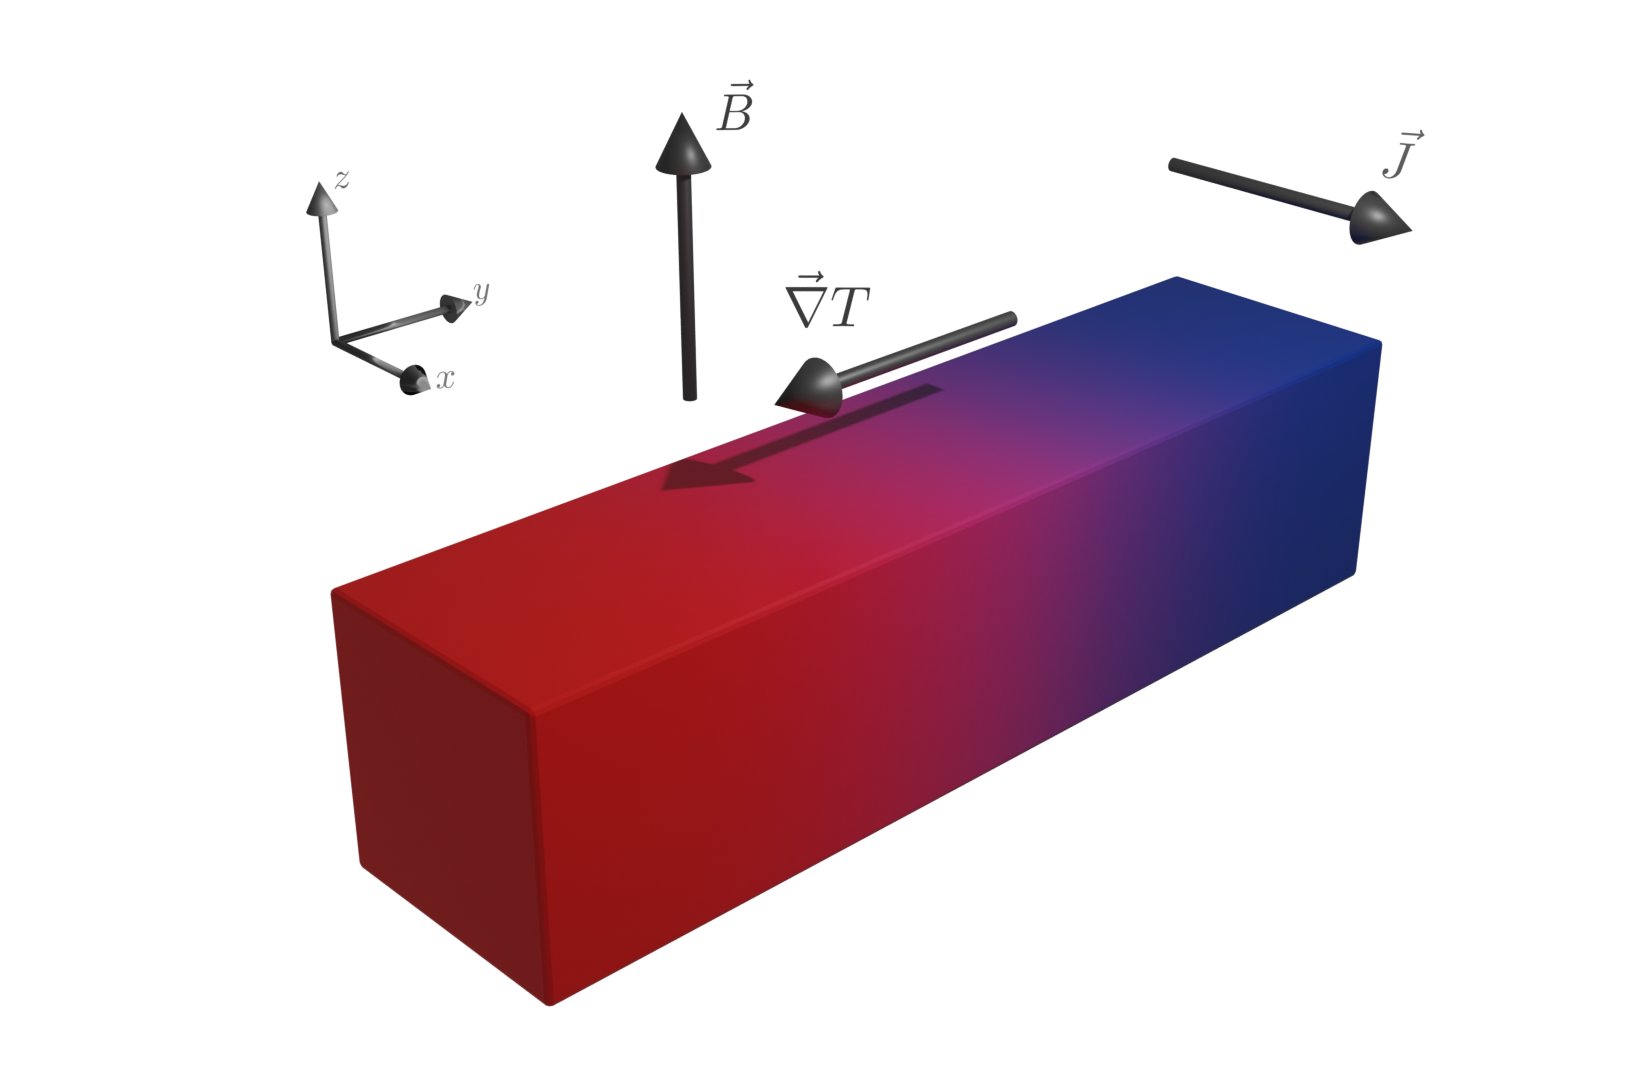
\includegraphics[width=0.7\textwidth]{figures/setup.png}
  \caption{Sketch of the geometry used in the derivation. Note that we consider only bulk response, and the finite sample is only for illustration purposes. \label{fig:setup}}
\end{figure}
In the derivation of~\citeauthor{chernodubGenerationNernstCurrent2018}~\cite{chernodubGenerationNernstCurrent2018} the response
\begin{equation}
  \chi ^{xy} = \frac{e^2 v_F B}{18 \pi ^2 \hbar }
\end{equation}
was found, while the derivation of~\citeauthor{arjonaFingerprintsConformalAnomaly2019}~\cite{arjonaFingerprintsConformalAnomaly2019} found
\footnote{The paper is somewhat unclear on what is their final result, as there is some possible confusion related to the number of Landau levels included and whether one is including both or only one Dirac cone.
The above result is what is meant, to the best of our understanding.}
\begin{equation}
  \chi ^{xy} = \frac{e^2 v_F B}{4 \pi ^2 \hbar }.
\end{equation}

Recall the linear response from the Kubo formalism in Eq. (\ref{eq:current-luttinger-final}), found through Luttinger's approach.
\begin{equation}
  \label{eq:21}
  \braket{J^i}(t, \vec{r}) = \!\!
  \underbrace{
  \int\limits_{-\infty }^{\infty } \mathrm{d}t' \mathrm{d}\vec{r}' \!\!
  \int\limits_{-\infty }^{t'} \mathrm{d}t''
  \left\{
    \frac{-i v_F}{\hbar } \Theta (t-t')
    \Braket{
      [J^i(t, \vec{r}), T^{j 0} (t'', \vec{r}')]
    }
  \right\}
  }_{\chi^{ij}}
  \frac{- \partial _j' T(t', \vec{r}')}{T}.
\end{equation}
Fourier transforming now to the frequency and momentum domain, will be beneficial in our calculations.
As before, the non-perturbed system will be taken to be time and position invariant, such that the correlator in Eq. (\ref{eq:21}) can be taken to depend only on the differences $t-t''$ and $\vec{r} - \vec{r}' $.
Starting with Fourier transforming the position part, notice that the structure of Eq. (\ref{eq:21}) is
\[
  \braket{J^i}(\vec{r}) = \int \mathrm{d} \vec{r}' \chi (\vec{r} - \vec{r}') (-\partial _j' T(\vec{r}') /T),
\]
where the temporal parts were dropped for clarity.
This is a convolution, and the Fourier transform is thus simply given by the product of the two factors~\cite{rottmannMatematiskFormelsamling1995}.
\begin{equation}
  \braket{J^i}(\vec{q}) = -
  \chi (\vec{q}) (iq_j) T(\vec{q}) /T,
\end{equation}
where it was also used that the Fourier transform of a derivative gives the component of the variable.
Showing explicitly how to find the form of the response $\chi $ in momentum space is often overlooked in much literature, and as it does involve some finesse, we want to show it here.
This trick is courtesy of~\citeauthor{changLectureNotesManybody2018}~\cite{changLectureNotesManybody2018}.
By definition, the Fourier transform of the response is, where the variable of integration has been chosen to be $\vec{r}-\vec{r}'$ for later convenience,
\begin{align}
  \chi (\vec{q}) &= \int \mathrm{d}(\vec{r} - \vec{r}') e^{-i\vec{q}(\vec{r}-\vec{r}')} \chi (\vec{r} - \vec{r}')\\
                 &= \int \mathrm{d}(\vec{r} - \vec{r}') e^{-i\vec{q}(\vec{r}-\vec{r}')} C \Braket{
                   \left[
J^i (\vec{r}), T^{j 0}(\vec{r}')
                   \right]},\\
\end{align}
where $C$ denotes $t$-dependent prefactors and integrals over time are omitted, again for clarity of notation.
Note that
\begin{equation}
  \int \mathrm{d}(\vec{r} - \vec{r}') = \frac{1}{\mathcal{V}} \int \mathrm{d}\vec{r} \mathrm{d} \vec{r}',
\end{equation}
where $\mathcal{V}$ is the volume of the system.
Thus,
\begin{equation}
  \begin{split}
    \chi (\vec{q}) &= \frac{1}{\mathcal{V}} \int \mathrm{d}\vec{r} \mathrm{d}\vec{r}'
    e^{-i\vec{q}(\vec{r}-\vec{r}')}
    C \Braket{\left[
        J^i(\vec{r}), T^{j 0}(\vec{r}')
      \right]}\\
    &= \frac{C}{\mathcal{V}} \Braket{\left[ J^i(\vec{q}), T^{j 0}(-\vec{q}) \right]}.
  \end{split}
\end{equation}

Considering now the temporal part, the procedure is simpler.
The linear response still has the form of a convolution, as the response function is only dependent on the difference $t-t'$ by
\todo{Add indices to energy-momentum tensor}
\begin{equation}
  \chi (t-t') = \int\limits_{-\infty }^0 \mathrm{d} t'' \Theta (t - t')
  \Braket{\left[ J^i(t-t'), T^{j0}(t'') \right]},
\end{equation}
where $t''$ was shifted by $t' $, and then the translational invariance of the correlator was used.
In frequency space
\begin{align}
  \chi (\omega ) &= \int \mathrm{d} t e^{i \omega  t} \chi (t)\\
                 &= \int \mathrm{d} t e^{i \omega  t} \int\limits_{-\infty  }^0 \mathrm{d} t''
                   \Theta (t) \Braket{\left[ J^i(t), T^{j 0}(t'') \right]}.
\end{align}
In frequency and momentum space the response function is thus
\begin{equation}\label{eq:22}
  \chi ^{ij} (w, \vec{q}) =
  \frac{-iv_F}{\mathcal{V} \hbar }
  \int \mathrm{d}t e^{i\omega t}
  \int\limits_{-\infty }^{0} \mathrm{d}t'
  \Theta (t)
  \Braket{\left[
      J^i(t, \vec{q}), T^{j 0}(t', -\vec{q})
    \right]}.
\end{equation}

% \section{Complications and considerations}
\section{General remarks}
Before beginning the computation, we here briefly mention some complications and considerations important to our result.
Firstly we discuss how the charge current form a Kubo calculation relate to experimentally measurable currents.
Secondly we discuss the ambiguity related to the energy-momentum tensor.

\subsection{Transport and magnetization}
\label{sec:transport-magnetization}
Recall that we generally define the transport coeffieicents (Eq.~\eqref{eq:17})
\[
J^i = -e L_{ij}^{11} \left[
          E_j - T \nabla_j \frac{\mu}{T}
  \right] - e L^{12}_{ij} T \nabla_j \frac{1}{T},
\]
where \( J^i \) is the electrical current.
In our work, we focus on the \( L^{12} \) coefficient, however the following discussion is valid also more generally.
The definition of transport currents becomes more subtle in systems with broken time-reversal symmetry\cite{vanderwurffMagnetovorticalThermoelectricTransport2019, chernodubThermalTransportGeometry2021}.
In such systems, unobservable, circulating \emph{magnetization} currents arise.
These currents do not contribute to transport, but the Kubo treatment derives the local current, which in general also includes non-transporting currents.
Let
\begin{equation}
  \label{eq:23}
  \vec{J} = \vec{J}_{\text{tr}} + \vec{J}_M,
\end{equation}
where \( \vec{J} \) is the total local current, \( \vec{J}_{\text{tr}} \) is the transport current, and \( \vec{J}_M \) is the circulating magnetization current.
The Kubo formalism generally gives the response to the total local current, \( \chi \);
we are more interested in the experimentally measurable transport response \( L_{ij}^{12} \), related to our Kubo result as
\cite{chernodubThermalTransportGeometry2021}
\begin{equation}
  \label{eq:24}
  L^{12}_{ij} = -\chi_{ij} /e + \epsilon^{ijl} M_l,
\end{equation}
with \( M_l \) the magnetization.
For zero chemical potential, however, these magnetization currents have been shown to go to zero as \( T \to 0 \) \cite{vanderwurffMagnetovorticalThermoelectricTransport2019}.
The result from the Kubo calculation is therefore the actual transport current.


\subsection{Comment on the energy-momentum tensor}
There is some ambiguity with regards to the definition of the energy-momentum tensor\cites{kachelriessQuantumFieldsHubble2018}{chernodubThermalTransportGeometry2021}{vanderwurffMagnetovorticalThermoelectricTransport2019}{forgerCurrentsEnergyMomentumTensor2004}.
The \emph{canonical} energy-momentum tensor, derived from Lagrangian mechanics, is defined as
\begin{equation}
	T^{\mu \nu } = \frac{\partial \mathcal{L}}{\partial \partial _{\mu } \psi_i } \partial ^{\nu } \psi_i - \eta^{\mu \nu } \mathcal{L}.
\end{equation}
On the other hand, from general relativity, the \emph{dynamical} energy-momentum tensor is defined by the variation of the (matter) action with respect to the metric\cite{kachelriessQuantumFieldsHubble2018}
\todo{Signs depend on choice of g}
\begin{equation}
	T^{\mu \nu} = \frac{2}{\sqrt{g} } \frac{\delta S}{\delta g_{\mu \nu}}.
\end{equation}
Immediately, we see that the first definition is in general not symmetric, while the latter is, as the metric is always symmetric \footnote{something with torsion never}.
As the energy-momentum tensor is an observable, this presents a problem:
how should the tensor be defined?
This issue is not trivial, and has puzzled physicists for decades\cite{forgerCurrentsEnergyMomentumTensor2004}.

Superficially, we make the following observations.
The \emph{defining} property of the energy-momentum tensor is its conservation law
\begin{equation}
  \label{eq:78}
  \partial_{\mu} T^{\mu \nu} = 0,
\end{equation}
on a flat manifold.
This, of course, only defines the tensor up to a total divergence.
Denote by \( \hat{T}^{\mu \nu} \) the \emph{canonical} energy-momentum tensor.
We can then define another tensor
\begin{equation}
  \label{eq:79}
  T^{\mu\nu} = \hat{T}^{\mu \nu} + \partial_{\alpha} S^{\alpha \mu \nu}.
\end{equation}
By letting the additional term be anti-symmetric \( S^{\alpha \mu \nu} = - S^{\mu \alpha \nu}\), it is divergence free.
This is easily shown as follows:
\begin{align}
  \label{eq:80}
  \partial_{\mu} \partial_{\alpha} S^{\alpha \mu \nu} &= - \partial_{\mu} \partial_{\alpha} S^{\mu \alpha \nu}\\
                                                        &= - \partial_{\alpha} \partial_{\mu} S^{\mu \alpha \nu}\\
  &= -\partial_{\mu} \partial_{\alpha} S^{\alpha \mu \nu},
\end{align}
where we used the commutation of partial derivatives and relabelling of the dummy indices \( \mu, \lambda \).
By an appropriate choice of \( S^{\alpha \mu \nu} \) the canonical energy-momentum tensor may be symmetrized, importantly while still abiding the conservation law.
The correction that symmetrizes the energy-momentum tensor is known as the ``Belifnante tensor'', which for the Dirac Lagrangian is\cite{chernodubThermalTransportGeometry2021}
\begin{equation}
  \label{eq:81}
  S^{\alpha \mu \nu} = \frac{1}{8} \bar{\Psi}\left[ \gamma^{\alpha}, \sigma^{\mu\nu} \right] \Psi,
\end{equation}
which gives
\begin{equation}
  \label{eq:82}
  T^{\mu \nu} = \frac{1}{4} \bar{\Psi} (\gamma^{\mu} D^{\nu} + \gamma^{\nu} D^{\mu}) \Psi.
\end{equation}
Which, in the case of the Dirac Lagrangian, so happens to correspond to the naive symmetrization
\begin{equation}
  \label{eq:83}
  T^{\mu\nu}_s = \frac{T^{\mu \nu} + T^{\nu \mu}}{2}.
\end{equation}

It is also instructive for our work to consider a more naive line of reasoning.
The energy-momentum tensor is used in this work through its conservation law Eq.~\eqref{eq:78}, whose first component gives the conservation of energy.
Writing it out explicitly
\begin{equation}
  \label{eq:84}
  \partial_0T^{00} + \partial_i T^{i0} = \partial_0 \epsilon + \partial_i j^i_{\epsilon} = 0,
\end{equation}
with \( \epsilon \) the energy density and \( \vec{j}_{\epsilon} \) the energy density current, the question is really seen to be finding the energy density current, ignoring all formal arguments about the energy-momentum tensor in a general context.
Using such a line of reasoning \textcite{vanderwurffMagnetovorticalThermoelectricTransport2019} argued that the appropriate form of the energy-momentum tensor that should be used in linear response calculations of Dirac material systems, is the unsymmetrized canonical tensor.
In this work, we will therefore use the canonical energy-momentum tensor, as opposed to the symmetric form used in the linear response calculation of an untitled cone done by \textcite{arjonaFingerprintsConformalAnomaly2019}.
In the untilted case, the two definitions give the same contribution, while for a titled cone, the response from the two definitions differ.

In the case of an untilted system, the components of interest of the canonical energy-momentum tensor reads
\begin{subequations}
\begin{align}
  T^{y 0} &= \frac{s i}{4}
  \left[
  \phi^{\dagger} \sigma_y \partial_{0} \phi - \partial_0 \phi^{\dagger} \sigma_y \phi
  \right],\\
  T^{0 y} &= \frac{v_F}{4}
  \left[
  \phi^{\dagger} p_y \phi - p_y \phi^{\dagger} \phi
  \right].
\end{align}
\end{subequations}
The symmetrized energy-momentum tensor used by \textcite{arjonaFingerprintsConformalAnomaly2019}
\begin{equation}
  T_s^{y 0} = \frac{T^{y 0} + T^{0 y}}{2}.
\end{equation}
The response was found to be
\begin{equation}
  \chi = [\dots] \sum\limits_{\underset{N=M-1}{m,n}}^{} \int \mathrm{d} \kappa_z (F^{(1)} + F^{(2)}) \alpha_{\kappa_z m s}^2,
\end{equation}
with \( [\dots] \) prefactors not relevant here, and \( F^{(i)},\, i=1,2 \) the contribution from \( T^{y0} \) and \( T^{y 0} \), respectively.
They are
\begin{align}
  F^{(1)} &= \epsilon_{\kappa_z m s} + \epsilon_{\kappa_z n s},\\
  F^{(2)} &= s \alpha_{\kappa_z n s} \sqrt{M-1} + \frac{s \sqrt{M}}{\alpha_{\kappa_z m s}},
\end{align}
where we have used the dimensionless
\[
  \epsilon_{\kappa_z m s} = \frac{\sqrt{2eB}}{v_{F}} E_{k_z m s}, \quad \kappa_z = \sqrt{2 e B} k_z.
\]
Using the explicit form of the normalization factor
\[
  \alpha_{k_z m s} = - \frac{s \sqrt{M}}{\epsilon_{m} - s \kappa_z},
\]
and energy eigenstates
\[
  \epsilon_m = \sign (m) \sqrt{M + \kappa_{z}^2},
\]
it is not difficult to show that
\begin{equation}
  F^{(2)} = \epsilon_{\kappa_z m s} + \epsilon_{\kappa_z n s} = F^{(1)}.
\end{equation}

Tilting parallel to the magnetic field does not alter the eigenstates, it only changes the eigenvalues by a factor \( t_{\parallel} v_F k_z \) \cites{yuPredictedUnusualMagnetoresponse2016,tchoumakovMagneticFieldInducedRelativisticProperties2016}, as we will show later.
The results from the untilted case may thus be applied directly, with rescaled energies.
As the normalization factor \( \alpha_{\kappa_z m s} \) is invariant under the tilt, \( F^{(2)} \) does not change.
However, \( F^{(1)} \) changes to
\begin{equation}
  \label{eq:163}
  F^{(1)} = \epsilon_{\kappa_z m s} + \epsilon_{\kappa_z n s} = \epsilon^0_{\kappa_z m s} + \epsilon^0_{\kappa_z n s} + 2 \kappa_z t_{\parallel},
\end{equation}
where \( \epsilon^0_{\kappa_z m s} \) is the energy levels of the untilted system.
The last term in Eq.~\eqref{163} gives a non-zero contribution to the total response, and so the results for a tilted cone is generally dependent on the choice of the energy-momentum tensor.


\todo{Decide dimless or dimfull quantities}
